\documentclass{article}
\usepackage{graphicx} % Required for inserting images

\begin{document}

\title{eBuy}
\maketitle
\section{Classe Post}
\subsection{Operazioni}

\begin{enumerate}
    \item \texttt{ChiudiAsta()}
    
    \textbf{pre:} \\ 
            nessuna    \\
    \textbf{post:} 
    
    \begin{itemize}
        \item Se \texttt{this} è un'istanza \texttt{PostAsta}:
        
        Sia \texttt{scad} \texttt{this.IstanteScadenza}, sia \texttt{now} momento attuale (Giorno:Ora:Minuti:Secondi) attuale, non appena \texttt{scad=now} il post viene chiuso.
        
        Dato il link (\texttt{this}, \texttt{AstaConclusa}): \texttt{asta\_finita}
        
        Sia \texttt{pf} \texttt{this.UltimaOfferta}, viene impostato \texttt{AstaConclusa.PrezzoFinale=pf}
        
        Viene Creato un link (\texttt{AstaConclusa}, \texttt{UtenteRegistrato}): \texttt{utente\_vincitore} l'utente registrato è l'UtenteRegistrato del link (\texttt{this}, \texttt{UtenteRegistrato}): {ultimo\_bidder}
        
        \item Se \texttt{this} è un istante \texttt{PostCompraSubito}:
        
        Quando un \texttt{UtenteRegistrato} invoca \texttt{CompraOggetto()} viene creato un link (\texttt{this}, \texttt{UtenteRegistrato}): \texttt{utente\_compratore}
    \end{itemize}
    
    \item \texttt{PostAsta:}
    
    \begin{enumerate}
        \item \texttt{AggiornaUltimoBidder()}
        
        \textbf{pre:} \\
        Ci sia almeno un link (\texttt{this}, \texttt{UtenteRegistrato}): \texttt{AstaInCorso} e \texttt{this.IstanteScadenza<now.}\\
        
        \textbf{post:}
        
        Sia \texttt{Aste} l'insieme dei link (\texttt{this}, \texttt{UtenteRegistrato}): \texttt{AstaInCorso}, ogni volta che un \texttt{UtenteRegistrato} usa l'operazione \texttt{UtenteRegistrato.ProponiBid()} viene aggiornato tale insieme.
        
        Viene creato un link (\texttt{this}, \texttt{UtenteRegistrato}): \texttt{ultimo\_bidder} con l'oggetto \texttt{UtenteRegistrato} per il quale \texttt{AstaInCorso.IstanteOfferta} sia maggiore di tutti
    \end{enumerate}
\end{enumerate}

\subsection{Vincoli Esterni:}\\

    \textbf{[V.PostAsta.IstanteScadeza]}\\
     Quando viene creato un nuovo oggetto di tipo \texttt{PostAsta} e viene specificato l'istante della scadenza questo deve essere maggiore del tempo in cui il post viene creato



\section{Classe UtenteRegistrato}

\subsection{Operazioni:}

\begin{enumerate}
    \item \texttt{CreaNuovoPost(an: Intero):}
    
    \textbf{pre:}\\ \texttt{this.DataRegistrazione<now} \\
    
    \textbf{post:} 
    
    Viene Creato un nuovo oggetto di tipo \texttt{Post},
    
    Viene Creata un nuovo oggetto di tipo \texttt{Oggetto} ed il link (\texttt{Post},\texttt{Oggetto}): \texttt{post\_ogg}
    
    \item \texttt{ProponiBid(p:PostAsta):}
    
    \textbf{pre:}\\ nessuna\\
    
    \textbf{post:}
    
    Sia \texttt{p} un \texttt{PostAsta} con \texttt{p.IstanteScadenza>now}
    
    Viene creato un link (\texttt{this}, \texttt{p}): \texttt{AstaInCorso}
    
    Viene impostato \texttt{AstaInCorso.OffertaAttuale} come \texttt{p.UltimaOfferta+p.AmmontareRialzi}
    
    \item \texttt{CompraOggetto(p:PostCompraSubito)}
    
    \textbf{pre:} nessuna
    
    \textbf{post:}
    
    Sia \texttt{p} un \texttt{PostCompraSubito} con \texttt{p.Attivo = True}
    
    Viene impostato \texttt{p.Attivo= False} e chiamato \texttt{p.ChiudiVendita()}
\end{enumerate}

\subsection{Vincoli Esterni:}\\
\begin{enumerate}
    \item \textbf{[V.UtenteRegistrato.DataRegistrazione]}\\
    {UtenteRegistrato.DataRegistrazione<=now.}
    \item \textbf{[V.UtenteRegistrato.CreaNuovoPost()]}\\
    Se \texttt{UtenteRegistrato} usa la funzione \texttt{UtenteRegistrato.CreaNuovoPost()}, non può usare l'operazione \texttt{UtenteRegistrato.ProponiBid()} sull'oggetto creato con \texttt{UtenteRegistrato.CreaNuovoPost()}, non può usare l'operazione \texttt{UtenteRegistrato.ComoraOggetto()} sull'oggetto creato con \texttt{UtenteRegistrato.CreaNuovoPost()}
\end{enumerate}

    
    

\newpage
\section{Specifica Tipi di Dato}

\begin{enumerate}
    \item \textbf{PagamentoAccettato}
    
    \texttt{PagamentoAccettato=\{"Bonifico","Carta di Credito","Bonifico-Carta di Credito"\}}
    
    \item \textbf{StatoOggetto}
    
    \texttt{StatoOggetto=\{"Nuovo","Usato"\}}
    
    \item \textbf{DataIstante}
    
    \texttt{DataIstante=\{"Data":Data; "Istante":Time\}}
    
    \item \textbf{CondizioniOggetto}
    
    \texttt{CondizioniOggetto=\{"ottimo", "buono", "discreto", "da sistemare"\}}
\end{enumerate}
\newpage
\section{UML}
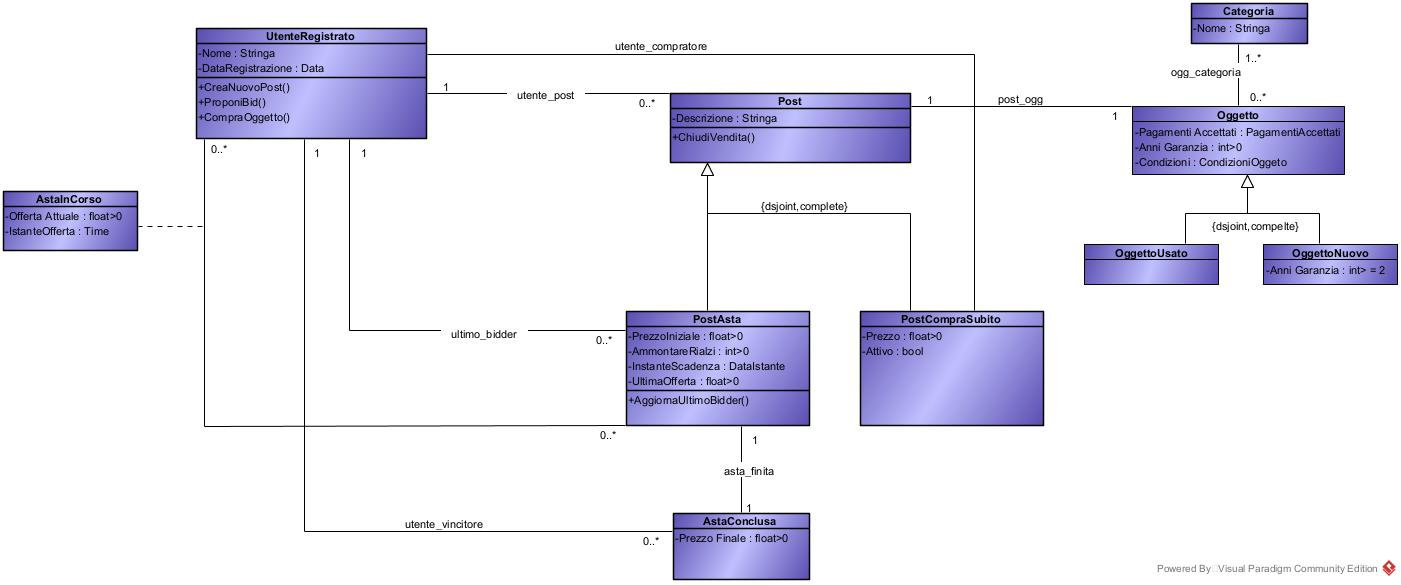
\includegraphics[width=\textwidth]{UML.jpg}
\end{document}
